\documentclass[review]{elsarticle}
\usepackage[utf8]{inputenc} 
\usepackage{lineno,hyperref}
\usepackage{tabu}
\usepackage{float}
\usepackage{tabularx}
\usepackage{subfigure}
\usepackage[fleqn]{amsmath}
\modulolinenumbers[5]

\usepackage{framed}
\usepackage{multicol} % Multiple columns environment

\usepackage{nomencl} % Nomenclature package
\makenomenclature
\setlength{\nomitemsep}{0pt}

\newcommand{\nomunit}[1]{%
  \renewcommand{\nomentryend}{\hspace*{\fill}#1}%
}

\renewcommand\nomgroup[1]{% 
  \item[\bfseries
  \ifstrequal{#1}{A}{Symbols}{%
  \ifstrequal{#1}{B}{Greek symbols}{%
  \ifstrequal{#1}{C}{Abbreviations}{}}}%
]}

\journal{Energy} 

%%%%%%%%%%%%%%%%%%%%%%%
%% Elsevier bibliography styles
%%%%%%%%%%%%%%%%%%%%%%%
%% To change the style, put a % in front of the second line of the current style and
%% remove the % from the second line of the style you would like to use.
%%%%%%%%%%%%%%%%%%%%%%%

%% Numbered
%\bibliographystyle{model1-num-names}

%% Numbered without titles
%\bibliographystyle{model1a-num-names}

%% Harvard
%\bibliographystyle{model2-names.bst}\biboptions{authoryear}

%% Vancouver numbered
%\usepackage{numcompress}\bibliographystyle{model3-num-names}

%% Vancouver name/year
%\usepackage{numcompress}\bibliographystyle{model4-names}\biboptions{authoryear}

%% APA style
%\bibliographystyle{model5-names}\biboptions{authoryear}

%% AMA style
%\usepackage{numcompress}\bibliographystyle{model6-num-names}

%% `Elsevier LaTeX' style
\bibliographystyle{elsarticle-num}
%%%%%%%%%%%%%%%%%%%%%%

\begin{document}

\begin{frontmatter}

\title{Numerical investigation of low-load operation of a subcritical power boiler using CFD and process modelling}

%% Group authors per affiliation:
\author{B.T. Rawlins}
\author{R. Laubscher\corref{mycorrespondingauthor}}
\cortext[mycorrespondingauthor]{Corresponding author}
\ead{ryno.laubscher@uct.ac.za}
\author{P. Rousseau}
\address{Department of Mechanical Engineering, Applied Thermal-Fluid Process Modeling Research Unit, University of Cape Town, Library Rd, Rondebosch, Cape Town, 7701, South Africa}
\address{$^*$ Department of Mechanical Engineering, Stellenbosch University, Stellenbosch Central, Stellenbosch, 7599, South-Africa}

\begin{abstract}
This paper uses co-simulation techniques which incorporate a computational fluid dynamic (CFD) model together with a process level model to investigate the low-load operation of a 620 $MWe$ sub-critical boiler. A 1D discretized two-phase model of the water/steam circuit of the furnace, the radiant superheaters (SH) and the convective/back pass heat exchangers was developed. This was coupled with a detailed CFD model incorporating the furnace and radiant superheaters using an Eulerian-Eulerian reference frame. The coupled model is used to investigate the combustion stability, the water/steam side effects and the radiant heat exchanger operational limits for six burner firing arrangements for a minimal boiler load of 32 \%. The results show that certain firing arrangements can lead to a high possibility of fire-side corrosion and the over-heating of heat exchanging components. Based on the numerical simulations carried out in terms of obtaining combustion stability, a favourable boiler utilization efficiency and the safe operation of heat exchanging components, a mixed firing arrangement accompanied with a higher secondary air (SA) mass flow-rate for non-firing burners was selected as the best case for the boiler under investigation.
\end{abstract}

\begin{keyword}
CFD\sep Boiler \sep Low-load operation \sep Co-simulation
\end{keyword}
\newpage
\end{frontmatter}

\printnomenclature

\nomenclature[A]{$A$}{Area \nomunit{$m^2$}}
\nomenclature[A]{$A_p$}{Particle surface area \nomunit{$m^2$}}
\nomenclature[A]{$A_{pn}$}{Projected particle surface area \nomunit{$m^2$}}
\nomenclature[A]{$A_{c}$}{Carbon pre-exponential factor \nomunit{$s^{-1}$}}
\nomenclature[A]{$A_{vol}$}{Volatile pre-exponential factor \nomunit{$s^{-1}$}}
\nomenclature[A]{$d_p$}{Particle diameter \nomunit{$m$}}
\nomenclature[A]{$E$}{Fluid total energy \nomunit{$J/kg$}}
\nomenclature[A]{$E_{a,c}$}{Carbon activation energy \nomunit{$J/kmol$}}
\nomenclature[A]{$E_{a,vol}$}{Volatile activation energy \nomunit{$J/kmol$}}
\nomenclature[A]{$E_p$}{Particle emission power \nomunit{$W/m^3$}}
\nomenclature[A]{$f_{heat}$}{Near surface char oxidation fraction \nomunit{$-$}}
\nomenclature[A]{$f_{p}$}{Forward scattering factor \nomunit{$-$}}
\nomenclature[A]{$G$}{Incident radiation \nomunit{$W/m^2$}}
\nomenclature[A]{$g$}{Gravitational constant \nomunit{$m/s^2$}}
\nomenclature[A]{$h_{fg}$}{Enthalpy of evaporation \nomunit{$J/kg$}}
\nomenclature[A]{$h_M$}{Mixture enthalpy \nomunit{$J/kg$}}
\nomenclature[A]{$h_{rxn}$}{Enthalpy of reaction \nomunit{$J/kg$}}
\nomenclature[A]{$J_k$ }{Species diffusion flux \nomunit{$m^2/s$}}
\nomenclature[A]{$m_{0,vol}$}{Original mass of volatiles \nomunit{$kg$}}
\nomenclature[A]{$m_{char}$}{Mass of carbon \nomunit{$kg$}}
\nomenclature[A]{$m_{evap}$}{Mass of moisture \nomunit{$kg$}}
\nomenclature[A]{$m_{vol}$}{Mass of volatiles \nomunit{$kg$}}
\nomenclature[A]{$N_{p}$}{Number of particles \nomunit{$-$}}
\nomenclature[A]{$P$}{Perimeter \nomunit{$m$}}
\nomenclature[A]{$p$}{Pressure \nomunit{$Pa$}}
\nomenclature[A]{$p_{O_{2}}$}{Partial pressure of $O_2$ \nomunit{$Pa$}}
\nomenclature[A]{$\dot{Q}_{conv}$}{Convective heat transfer rate \nomunit{$W$}}
\nomenclature[A]{$\dot{Q}_{rad}$}{Radiative heat transfer rate \nomunit{$W$}}
\nomenclature[A]{$\dot{Q}_{w}$}{Wall heat transfer rate \nomunit{$W$}}
\nomenclature[A]{$R$}{Universal gas constant \nomunit{$J/molK$}}
\nomenclature[A]{$R_{c}$}{Carbon reaction rate \nomunit{$s^{-1}$}}
\nomenclature[A]{$R_{diff}$}{Diffusion reaction rate \nomunit{$s^{-1}$}}
\nomenclature[A]{$R_{vol}$}{Volatile reaction rate \nomunit{$s^{-1}$}}
\nomenclature[A]{$T_g$}{Gas temperature \nomunit{$K$}}
\nomenclature[A]{$T_p$}{Particle temperature \nomunit{$K$}}
\nomenclature[A]{$t$}{Time \nomunit{$s$}}
\nomenclature[A]{$u$}{Velocity \nomunit{$m/s$}}
\nomenclature[A]{$V$}{Volume \nomunit{$m^3$}}
\nomenclature[A]{$Y_k$}{Species mass fraction \nomunit{$kg/kg$}}
\nomenclature[A]{$x$}{Quality \nomunit{$-$}}
\nomenclature[B]{$\alpha_g$}{Gas absorption coefficient \nomunit{$m^{-1}$}}
\nomenclature[B]{$\alpha_H$}{Mixture void fraction \nomunit{$-$}}
\nomenclature[B]{$\alpha_p$}{Particle absorption coefficient \nomunit{$m^{-1}$}}
\nomenclature[B]{$\epsilon_p$}{Particle emissivity \nomunit{$-$}}
\nomenclature[B]{$\rho$}{Gas density \nomunit{$kg/m^3$}}
\nomenclature[B]{$\rho_{eff}$}{Effective density \nomunit{$kg/m^3$}}
\nomenclature[B]{$\rho_g$}{Gas density \nomunit{$kg/m^3$}}
\nomenclature[B]{$\rho_l$}{Liquid density \nomunit{$kg/m^3$}}
\nomenclature[B]{$\rho_M$}{Mixture density \nomunit{$kg/m^3$}}
\nomenclature[B]{$\rho_p$}{Particle density \nomunit{$kg/m^3$}}
\nomenclature[B]{$\sigma_{SB}$}{Stefan-Boltzmann constant \nomunit{$W/m^2K^4$}}
\nomenclature[B]{$\sigma_{p}$}{Particle scattering coefficient \nomunit{$m^{-1}$}}
\nomenclature[B]{$\phi$}{Scalar variable \nomunit{$-$}}
\nomenclature[C]{$MCR$}{Maximum continuous rating}
\nomenclature[C]{$CFPP$}{Coal fired power plant}
\nomenclature[C]{$CFD$}{Computational fluid dynamics}
\nomenclature[C]{$SH$}{Superheater}
\nomenclature[C]{$EE$}{Eulerian-Eulerian}
\nomenclature[C]{$WSGGM$}{Weighted sum of gray gas model}
\nomenclature[C]{$RTE$}{Radiative transport equation}
\nomenclature[C]{$HHV$}{Higher heating value}
\nomenclature[C]{$DAF$}{Dry ash free}
\nomenclature[C]{$AR$}{As-received}
\nomenclature[C]{$PA$}{Primary air}
\nomenclature[C]{$SA-AH$}{Secondary air - air heater}
\nomenclature[C]{$SA$}{Secondary air}
\nomenclature[C]{$RH$}{Reheater}
\nomenclature[C]{$ATT$}{Attemperator}
\nomenclature[C]{$EC$}{Economiser}
\nomenclature{\mbox{}}{}
\linenumbers
\section{Introduction}
The use of coal-fired power plants (CFPP) to provide electricity generation is intended to be phased out in order to mitigate the ingress of climate change. However, the switch to sustainable generation sources poses great challenges for developing countries due to the long transition times and costs involved \cite{ugum2019}. Due to the abundance of coal resource present in Southern Africa, CFPPs are the dominant power generation source, with approximately 80 \% of the energy needs being met using CFPPs \cite{eskom}. The promising integration of renewable energy and the decommissioning of old CFPPs in Southern Africa, will push these plants from a primarily base load operation to a mid-merit/flexible operating protocol. The switch to flexible operation will inherently mean CFPPs will need to operate at low-loads for continuous time periods. 

Mathematical models that can accurately capture the thermal response of boilers at varying loads can be used to determine the safe and efficient operating limits \cite{Laubscher2019b}. Since, the long term deviation from design conditions can lead to operational inefficiencies affecting combustion stability \cite{Hernik2020}, an increase in harmful emissions \cite{Chang2021} and the localised overheating of heat exchangers due to insufficient cooling being provided by the internal working fluid \cite{Modlinski2019}.

The full scale testing or experimentation of CFPPs is deemed to expensive to pursue, thus the use of computational fluid dynamics (CFD) allows for the modelling of a full-scale CFPPs, at steady-state, to be investigated at various loads circumventing the use of time-consuming and costly field tests. CFD simulations have been successfully used to model a variety of CFPP boiler types (\cite{Laubscher2019a}, \cite{Gu2020}) and cover various aspects such as pollution control (\cite{Du2017},\cite{Fan2001}), gas-solid flow effects (\cite{Chen2017}) and boiler retrofitting (\citep{Gu2020}, \cite{He2007}).

Recent CFD studies investigating low-load operation of CFPP boilers have focused on the combustion stability, harmful emissions and the gas flow-solid flow interactions \cite{Jiang2021}. The works of Belosevic et al \citep{Belosevic2019a} found that the low-load operation of boiler considerably affect the flow and temperature fields, the flame geometry, chemical reactions and concentrations of combustion products.

Hernik et al \cite{Hernik2020} investigated the effects of using different mill system configurations at a minimum boiler load of 40 \%. The most favourable mill system configuration was selected based on the case that exhibited suitable combustion stability and emission of harmful substances. Similarly, Chang et al \citep{Chang2021} investigated the various firing arrangements of a 630 $MWe$ tangentially fired boiler. A burner angle of -15 $^\circ$ was found to be the optimal arrangement resulting in the best compromise in combustion stability and lower emissions. The aforementioned reseacrh specifically investigated combustion and gas-side effects. However, to the best the authors' knowledge, no integration of 1-D process model has been used to investigate the steam side operational performance of a CFPP boiler at low-load.

The use of a 1-D process modelling approach have been used by researchers to investigate the water and gas side heat transfer interactions. These studies are usually used to investigate a transient event, such as a sudden disturbance, start-up or boiler load ramping \cite{Alobaid2017}. Due to the non-uniformities found in CFPP furnaces which are composed of complex combustion dynamics, gas-solid interactions and  radiation heat transfer phenomena, 1-D process models can not resolve the fireside with sufficient accuracy, but can adequately resolve the waterside energy and momentum transport in a computationally inexpensive manner. 

The use of coupled simulations has proven to solve the deficiencies of a full 1-D process model by coupling the fireside CFD results to a 1-D water side model. Some recent papers that investigated boiler operations using a co-simulation approach are: Laubscher and Rousseau \cite{Laubscher2020} conducted a comprehensive numerical study on the impact of particle radiation properties for high ash coals using ANSYS Fluent v19.2\textsuperscript{\textregistered} and Flownex SE\textsuperscript{\textregistered}. Yu et al \cite{Yu2019} used a coupled simulation methodology to estimate the superheater (SH) metal temperatures of a 660 $MWe$ tangentially-fired coal boiler.

The goal of the current work is to investigate the effect of burner firing configuration on various process parameters such as steam temperatures, spray water flow-rates and metal temperatures. The current work proposes the use of CFD modelling  to investigate the low-load gas-side effects at various firing conditions for a 620 $MWe$ two-pass sub-critical boiler. For the current work CFD gas-side results are coupled to a comprehensive process model of the case study boilers water side. 

The model was simulated for a boiler load of 32 $\%$  with 6 various firing combinations. To establish the accuracy of the CFD modelling approach a validation study was conducted for 100 $\%$, 80 $\%$ and 60 $\%$ maximum continuous rating (MCR) loads and compared to actual plant measurements to quantify the model accuracy, this is highlighted in section \ref{sec_model_valid} prior to the results of the low-load study. 

\section{Mathematical model}
In this section the modelling techniques used by the study are briefly discussed.
\subsection{Computational fluid dynamics modelling}
\subsubsection{Fluid flow, turbulence and combustion modelling}
The flue gas was modelled using a Eulerian framework. The species transport modelling approach was used to approximate the mixture of chemical species in the gas phase. This approach solves a species continuity equation for each constituent present in the mixture. To reduce the computational burden it was assumed that the various processes were in steady-state. The governing equations for the gas phase are written in their respective Reynolds averaged forms as follows;\\
Mass conservation:
\begin{equation}\label{eqn_RANS_mass}
\frac{\partial}{\partial x_{i}}(\rho \bar{u}_{i})=S_{m}.
\end{equation}
Momentum conservation:
\begin{equation}\label{eqn_momentum}
\frac{\partial}{\partial x_{i}}(\rho_{eff} u_{i}u_{j})+\frac{\partial \overline{p}}{\partial x_{j}}=\frac{\partial}{\partial x_{i}}\left[\mu\left\{\frac{\partial u_{j}}{\partial x_{i}}+\frac{\partial u_{i}}{\partial x_{j}}-\frac{2}{3}\delta_{ij}\frac{\partial u_{i}}{\partial x_{i}}\right\}\right]+\frac{\partial}{\partial x_{i}}(-\rho\overline{u_{i}^{'}u_{j}^{'}})+S_m
\end{equation}
Energy conservation:
\begin{equation}\label{eqn_energy}
\frac{\partial }{\partial x_{i}} (u_{i}[\rho E+p])=\frac{\partial }{\partial x_{j}}\left[\lambda\frac{\partial T_{g}}{\partial x_{j}}\right] +S_{h}
\end{equation}
Species transport:
\begin{equation}\label{eqn_species}
\begin{split}
&\frac{\partial}{\partial x_{i}}(\rho u_{j}Y_{k})=-\frac{\partial}{\partial x_{j}}(\vec{J_{k}})+ \sum_r R_{j,r} + S_{k}\\
&k = 1,2,3...N
\end{split}
\end{equation}
To correctly account for the particle inertial effects on the gas phase convection, the model makes use of an effective density which is defined as follows;
\begin{equation} \label{eqn_eff_rho}
	\rho_{eff} = \frac{\rho \rho_p \left( \phi_{mp} + 1 \right)}{\rho \phi_{mp} + \rho_p}
\end{equation}

In the present study the realizable k-$\epsilon$ turbulence model was utilized to address the turbulence closure problem. This model has been successfully used by researchers (\cite{Belosevic2019a},\cite{Laubscher2019a} and \cite{Modlinski2019}), in modelling the effects of coal-fired swirl burners. The model generally produces higher accuracy results, when compared to the standard k-$\epsilon$ model, for problems incorporating swirling and separating flows.

The process of coal combustion comprises of four sequential steps. Namely, inert heating and evaporation of moisture, devolatilization, char oxidation and gas phase reactions. Equations (\ref{eqn_vol_rate}) and (\ref{eqn_vol_arrhenuis}) show the single rate kinetic model utilized in this study, to model the devolatilization process.
\begin{gather}
\frac{dm_{vol}}{dt} = R_{vol}(m_{0,vol}-m_{vol}) \label{eqn_vol_rate} \\
\begin{split}
&R_{vol} = A_{vol}exp\left(\frac{E_{a,vol}}{RT_p}\right)\\
&A_{vol} = 2\times10^5 [s^{-1}]\,\,\,\,\,\,\,\,\,\,E_{a,vol} = 6.7\times10^7 [J/kmol] \label{eqn_vol_arrhenuis}
\end{split}
\end{gather}

A devolatilization temperature of 553 [$K$] \citep{Ranade2015} along with the kinetic parameters (equation \ref{eqn_vol_arrhenuis}) of Sheng et al \cite{Sheng2004} were utilized in the present study. The char oxidation process is modelled using the diffusion-kinetics limited model developed by Baum and Street \cite{Baum1971}, which is given in equation (\ref{eqn_char_rate}). The product species of the char oxidation reaction was set to $CO$ as shown in equation (\ref{eqn_CO_reaction}). 
\begin{gather}
\frac{dm_{char}}{dt} = -A_p p_{O_{2}} \frac{R_{diff}R_c}{R_{diff} + R_c}  \label{eqn_char_rate}\\
C_{(s)}+0.5O_{2(g)}\to CO_{(g)} \label{eqn_CO_reaction}
\end{gather}
The diffusion and kinetic rates of equation (\ref{eqn_char_rate}) are defined in equations (\ref{eqn_char_diff_rate})  and (\ref{eqn_char_kin_rate}) with the kinetic parameters again taken from the works of Sheng et al \citep{Sheng2004}.
\begin{gather}
R_{diff} = \frac{5\times10^{-12}}{d_p} \left(\frac{T_g+T_p}{2}\right)^{0.75} \label{eqn_char_diff_rate}\\
\begin{split}
&R_{c} = A_{c}exp\left(\frac{E_{a,c}}{RT_p}\right)\\
&A_{c} = 0.0053 [kg/m^2sPa]\,\,\,\,\,\,\,\,\,\,E_{a,c} = 8.37\times10^7 [J/kmol]
\end{split}
 \label{eqn_char_kin_rate}
\end{gather}

The turbulence-chemistry interactions of the gas phase reactions were approximated using the eddy-dissipation-finite rate model used in ANSYS Fluent v19.5\textsuperscript{\textregistered} which calculates three rates, namely chemical reaction rate, turbulent production eddies dissipation rate and reaction eddies dissipation rate, and uses the minimum of the three for the source terms calculations. A description of the CFD gas phase reactions of the boiler under consideration, using the same coal, was previously published in the works of Laubscher and Rousseau \cite{Laubscher2019b}.

\subsubsection{Particle modelling}
The particles are modelled using a Eulerian reference frame, similar to the studies of Knaus et al \cite{Knaus2001a} and Benim et al \cite{Benim2005}, who both successfully used a Eulerian-Eulerain (EE) model to capture the characteristics of coal combustion and furnace heat transfer with adequate accuracy. The pseudo particle mass concentrations transported into the domain are modelled using the general scalar field transport equation with the necessary modifications to account for heat and mass transport \cite{Versteeg2007}. The pseudo-particles scalar fields are used to define the fuel characteristics based on the proximate analysis composition, namely consisting of moisture, volatile matter, fixed  carbon and ash. Each of the scalar field equations are given in Table \ref{tab_scalars}.

\begin{table}[h!]
\centering
\caption{Scalar field equation descriptions}\label{tab_scalars}  
\vspace{2mm}     
\begin{tabular}{lll}
\hline
Variable &Description& Transport equation \\
\hline
$\phi_{mp0}$ &Original/initial mass of particles& $\frac{\partial}{\partial x_{i}}(\rho u_{i} \phi_{mp0})=0$\\
$\phi_{M}$&Moisture present in particles&$\frac{\partial}{\partial x_{i}}(\rho u_{i} \phi_{M})=\frac{1}{V} \frac{dm_{evap}}{dt}$\\
$\phi_{VM}$&Volatile matter present in particles&  $\frac{\partial}{\partial x_{i}}(\rho u_{i} \phi_{VM})=\frac{1}{V}\frac{dm_{vol}}{dt}$\\
$\phi_{FC}$&Fixed carbon present in particles&$\frac{\partial}{\partial x_{i}}(\rho u_{i} \phi_{FC})=\frac{1}{V}\frac{dm_c}{dt}$\\
$\phi_{ASH}$&Ash present in particles&$\frac{\partial}{\partial x_{i}}(\rho u_{i} \phi_{ASH})=0$\\
$\phi_{hp}$&Enthalpy of particle&Equation \eqref{eqn_phi_hp}\\
\hline
\end{tabular}
\end{table}

The energy transport of the pseudo particle phase, is transported by defining a particle phase energy equation, which in turn uses the particle enthalpy.
\begin{equation}\label{eqn_phi_hp}
\frac{\partial}{\partial x_{i}}(\rho u_{i} \phi_{hp})=\left(f_{heat}\frac{dm_{c}}{dt}h_{rxn} + \dot{Q}_{rad} + \dot{Q}_{conv} - \frac{dm_{evap}}{dt}h_{fg}\right)\frac{1}{V}
\end{equation}

The equation accounts for all the processes associated with energy transport to the particle, namely convection $\left(\dot{Q}_{conv}\right)$, radiation $\left(\dot{Q}_{rad}\right)$, latent heat transport $\left(\frac{dm_{evap}}{dt}h_{fg}\right)$ and near surface char oxidation $\left(f_{heat}\frac{dm_{c}}{dt}h_{rxn}\right)$. This gives the model the ability to track the particle temperature in the domain, moving the model away from the thermal equilibrium approach incorporated by previous studies using an EE approach (\cite{Benim2005}, \cite{Vicente2003} and \cite{Cai2015}). The particle temperature is important in describing the sequential steps found in modelling combustion processes, especially at low boiler loads where mixing and ignition become problematic. To solve the additional transport equations and their source terms, C programs were developed.

\subsection{Heat transfer modelling modelling}
Radiation heat transfer is the dominant form of heat transfer found in industrial furnaces \citep{Basu2000} and is solved by applying the gray-participating-gas and particle medium configuration of the radiation transport equation (RTE) \cite{Modest2013} shown in equation (\ref{eqn_RTE}).
\begin{equation}\label{eqn_RTE}
\frac{d I(\vec{r},\hat{s})}{ds} = \alpha_g \frac{\sigma_{SB} T_{g}^4}{\pi}-(\alpha_g+\alpha_p+\sigma_p)I(\vec{r},\hat{s}) + \frac{\sigma_p}{4\pi}\int_{4\pi}I(\vec{r},\hat{s})\Phi d \Omega
\end{equation}
In the present work the RTE is solved using the P1 model. Ranade and Gupta \cite{Ranade2015} illustrated minimal differences between the two common radiation models (namely the P1 and discrete ordinates (DO)) for the resultant wall heat transfer rate values when modelling a 210 $MWe$ CFPP boiler. The P1 radiation model can include the effects of particle absorption ($\alpha_p$) and scattering ($\sigma_p$) as well as gas mixture absorption ($\alpha_g$). The P1 model transport variable is the incident radiation flux (G), and can be written for a particle laden domain as:
\begin{equation}
\begin{split}
&\frac{\partial}{\partial x_{i}}\left(\Gamma\frac{\partial G}{\partial x_{i}}\right)=\left(\alpha_g+\alpha_p\right)G-4\left(\alpha_g \sigma_{SB} T_{g}^4-\pi E_p \right)\\
&\Gamma = \frac{1}{\alpha_g+\alpha_p+\sigma_p}
\end{split}
\end{equation}

The flue gas absorptivity was calculated using the domain based weighted sum of gray gas model (WSGGM) using the coefficients determined by Smith et al \cite{Smith1982}. The WSGGM accounts for the radiation emitted by tri-atomic gases, namely $CO_2$, $H_2O$ and $SO_2$ present in the flue gas stream. The Eulerian description of the terms $\alpha_p$, $\sigma_p$ and $E_b$ are determined using the effective number of particles ($N_p = \rho \phi_{mp0} V / \left( \rho_p \pi \bar{d_p}^3 /6 \right)$) present in a cell. The equations for the radiative properties are given in equations (\ref{eqn_part_abs}) through (\ref{eqn_part_emisp}).
\begin{gather}
\alpha_p = \frac{\epsilon_p A_{pn}N_p}{V} \label{eqn_part_abs}\\
\sigma_p = \frac{(1-\epsilon_p)(1-f_p) A_{pn}N_p}{V} \label{eqn_part_scat} \\
E_p = \frac{\epsilon_p \sigma_{SB} T_p^4 A_{pn}N_p}{V}\label{eqn_part_emisp}
\end{gather}

It is important to note that variable properties for ($\epsilon_p$) and ($f_p$) were used, that are based on the correlations of Lockwood et al \cite{Lockwood1986} and Yin \citep{Yin2015} respectively.

\subsection{Process simulation model}
A 1D discretized model of the furnace evaporator, platen SH, final SH, and subsequent down stream heat exchangers was developed using Flownex SE\textsuperscript{\textregistered} 2021. The model simulates the internal convection heat transfer inside the tubes and the conduction through the tube walls. The model is able to simulate the attemperation flows and momentum transport through the steam/water circuit. The heat exchangers were modelled using a two-phase mixture approach, this assumes that the fluid properties, phase velocities and temperatures are uniform per cross-sectional area. The homogeneous mixture fraction and mixture density are defined in equations (\ref{eqn_vol_frac}) and (\ref{eqn_mix_rho}) respectively.
\begin{gather}
\alpha_H = \frac{\rho_l x}{\rho_lx + \rho_g(1-x)} \label{eqn_vol_frac}\\  
\rho_M = (1-\alpha_H)\rho_l + \alpha_H\rho_g \label{eqn_mix_rho}
\end{gather}
Applying the mixture density the following transport equations are solved per process model component;

\begin{equation}\label{eqn_mix_conti}
\frac{\partial}{\partial t}(\rho_M A)+\frac{\partial}{\partial s}(\rho_MAu) = 0
\end{equation}
\begin{equation}\label{eqn_mix_mom}
\frac{1}{A} \frac{\partial}{\partial t}(\rho_M A u)+\frac{1}{A} \frac{\partial}{\partial s}(\rho_M A u^2) = -\frac{\partial p}{\partial s}-\frac{\tau_W P}{A}- \rho_M g \frac{\partial z}{\partial s}
\end{equation}
\begin{equation}\label{eqn_mix_energy}
\begin{split}
&\frac{\partial}{\partial t}(\rho_Mh_M)+\frac{1}{A}\frac{\partial}{\partial s}(\rho_MAuh_M)+\frac{1}{2}\frac{\partial}{\partial s}(\rho_Mu^2)+\frac{1}{2A}\frac{\partial}{\partial s}(\rho_MAu^3)=\\&\frac{\partial p}{\partial t} + \frac{\dot{Q}_w}{V}-g\rho_Mu\frac{\partial z}{\partial s}
\end{split}
\end{equation}

The process model is used to determine the required attemperation flow rates in order to achieve the exit steam conditions, the boiler efficiency, and the steam generated for each case. The results of this model aid in determining the best firing combination of burner rows for continuous low-load operation, and the effects the various Cases have on the water-side of the boiler system.

\section{Case study boiler description \& set-up}
In this section the numerical model configuration, for both the CFD and process model, will be explained, covering the boiler geometry, the process model set-up, the various  modelling inputs (i.e. fuel characteristics and boundary conditions) and the numerical solution strategy.

\subsection{Geometry \& process model set-up}
The modelled  boiler is a two-pass sub-critical power boiler with a furnace depth of 13.77 [$m$], a width of 14.01 [$m$] and a height of 64 [$m$]. The CFD geometric model (of Figure \ref{fig_geometry}) makes use of a symmetry plane at half the width of the furnace. This was done to reduce the cell count of the numerical mesh. Both the platen and final SH are modelled as walls, with transverse pitches of 1.143 [$m$] and 0.8 [$m$] respectively. There are three levels of burners located on both the front and rear walls at heights of 11.9 [$m$], 19.3 [$m$] and 26 [$m$]. Figure \ref{fig_geometry} shows the modelled half of the furnace along with the locations of the platen SH, final SH, boundary walls (front, rear and side) and the domains outlet and inlets.\\
\begin{figure} [h!]
\centerline{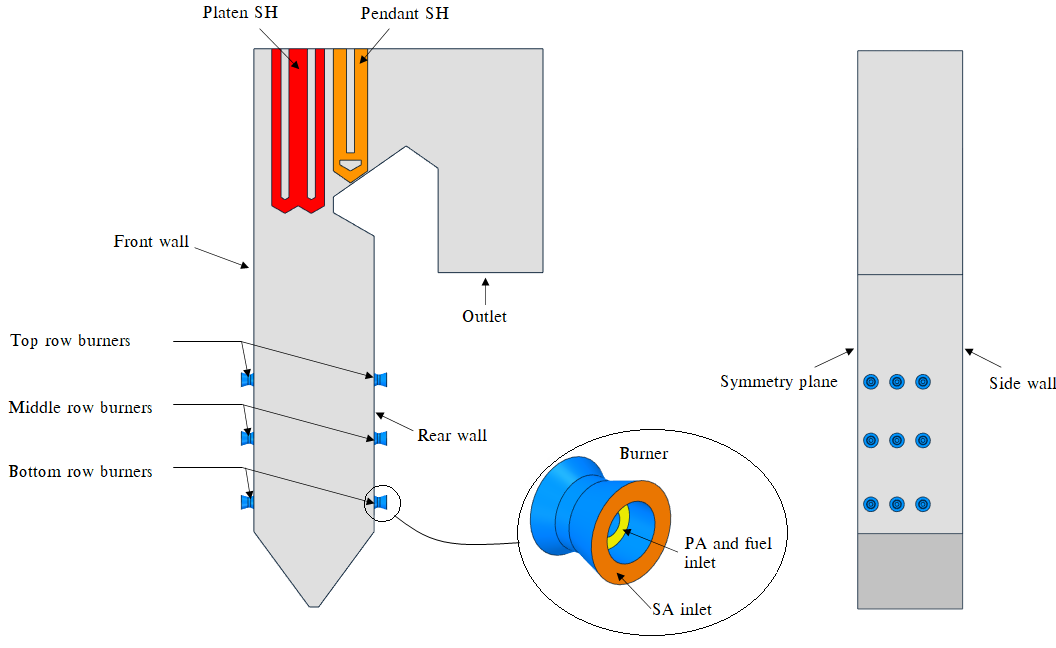
\includegraphics[scale=0.45]{GEOMETRY}}
\caption{Boiler geometry and layout}
\label{fig_geometry}
\end{figure}

The boiler furnace is fed by 6 mills, each supplying pulverised fuel and primary air (PA) mixture to a burner row consisting of 6 burners. This mixture is injected through the inner burner annulus while the secondary air (SA) is fed through the outer annulus as seen Figure \ref{fig_geometry}. 

The process model of the boiler configuration is shown in Figure \ref{fig_flownex}. The process model includes all the heat exchangers up to and downstream of the final SH, which include the secondary reheater (RH2), primary SH (SH1), primary reheater (RH1), economiser (EC) and the SA air heaters (SA-AH). The model includes all the relevant attemperators (ATT1, ATT2 and ATT-RH), inlets and outlets. The process model is used to determine the required attemperation flow-rates and water/steam side thermal response. The furnace water-walls are represented by a single lumped pipe flow component and forms part of the natural circulation system which include the downcomers and steam drum. As with the furnace walls, the platen and final SHs are similarly represented by a single lumped parameter pipe flow component, interconnected with nodes that introduce the attemperation flows to the water/steam side. 

The coupling interface between the simulation models are the heat exchanger external tube surfaces, namely the furnace, platen and final SH walls. The CFD heat loads are used as energy sources for these components as indicated in Figure \ref{fig_flownex}. Furthermore, the CFD flue-gas results (i.e. composition, mass flow and temperature) exiting the final SH are used as boundary inputs for the heat exchangers downstream of the final SH (SH3). The steam flow boundary values for the RH and EC sections are fixed mass inlet flows and temperatures with the corresponding outlets set to a fixed pressure.

\begin{figure}[h!]
\centering
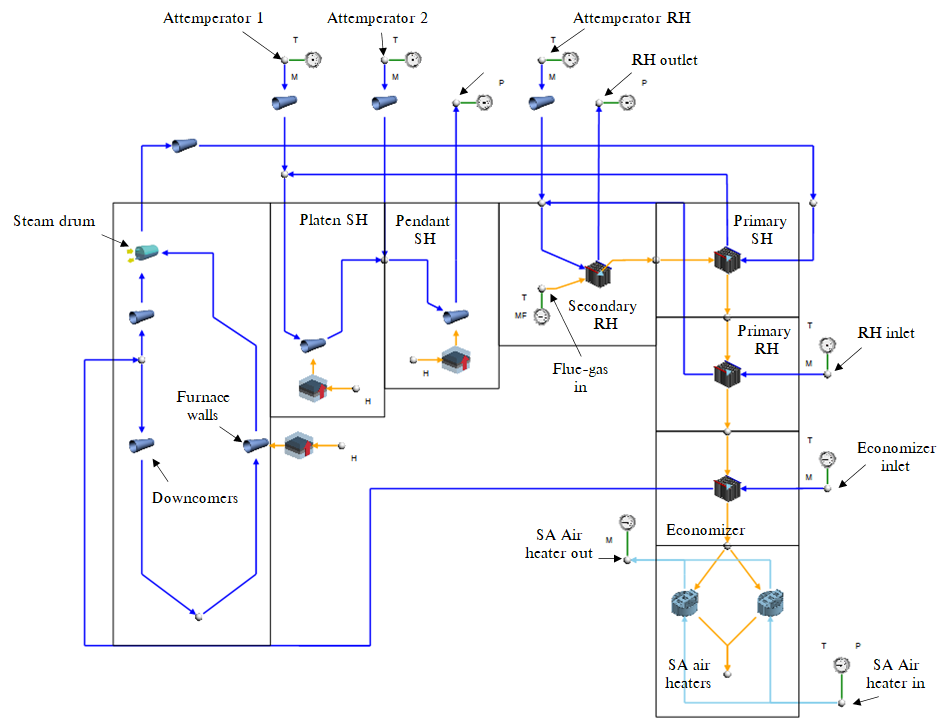
\includegraphics[scale=0.5]{FLOWNEX_SETUP}
\caption{Process model of boiler set-up including the downstream convective components using Flownex SE 2021}
\label{fig_flownex}
\end{figure}

\newpage
\subsection{Model inputs}
Table \ref{tbl_fuel} presents the coal characteristics utilized in the current study along with the fuels higher heating value (HHV).\\
\begin{table}[h!]
\centering
\caption{Utility boiler fuel characteristics}
\vspace{2mm}
\label{tbl_fuel}
{\tabulinesep=1.2mm
\begin{tabularx}{\textwidth}{p{0.45\textwidth} p{0.3\textwidth} l}
\hline
\textbf{Fuel constituent} & \textbf{Fraction} & \textbf{Unit}\\
\hline
\textit{Ultimate analysis - (DAF)} & \textit{-} & \textit{-}\\
Carbon & $0.7753$ & $kg/kg_{fuel}$\\
Hydrogen & $0.0415$ & $kg/kg_{fuel}$\\
Nitrogen & $0.0181$ & $kg/kg_{fuel}$\\
Oxygen & $0.1474$ & $kg/kg_{fuel}$\\
Sulphur & $0.0175$ & $kg/kg_{fuel}$\\
\textit{Proximate analysis - (AR)} & \textit{-} & \textit{-}\\
Fixed carbon & $0.340$ & $kg/kg_{fuel}$\\
Volatile matter & $0.196$ & $kg/kg_{fuel}$\\
Ash & $0.4090$ & $kg/kg_{fuel}$\\
Moisture & $0.0550$ & $kg/kg_{fuel}$\\
\hline
\textbf{Energy content - (DAF)} & \textbf{Value} &\\
\hline
Higher heating value & $15070$ & $kJ/kg_{fuel}$\\
\hline
\end{tabularx}}
\end{table}

For a 32 \% boiler load the current operational protocol is the to use the bottom front and rear burner rows to meet the low-load demand during start-up.  For this study six Cases are simulated in total with the following three burner firing configurations being investigated:
\begin{enumerate}
\item Bottom front and rear row burners are fired (Case 1 \& Case 4)
\item Middle front and rear row burners are fired (Case 2 \& Case 5)
\item Bottom front and middle rear row burners are fired (Case 3 \& Case 6)
\end{enumerate}

Typically 5 [$kg/s$] of air is fed through the non-firing burners, to ensure sufficient cooling of the burner and mixing of fuel and air in the combustion chamber. The result is a high air-fuel ratio in the furnace which leads to higher dry gas losses. to lower this loss, this study will investigate the affect of reducing the air-fuel ratio by lowering the non-firing burner SA flow-rate from 5 to 2.5 [$kg/s$].
Two permutations of the SA flow rate, at the non-firing burners, are used for each of the firing configurations mentioned above. Table \ref{tbl_case_inputs} shows the input conditions for Cases 1 to 6. The data is the result of a boilers mass and energy balance calculation.

\begin{table}[h!]
\centering
\caption{Case 1 to 6 model inputs on a per burner basis.}
\label{tbl_case_inputs}
\vspace{2mm}
{\tabulinesep=1.2mm
\begin{tabularx}{\textwidth}{p{0.45\textwidth} p{0.25\textwidth} l}
\hline
Active burners & \textbf{Cases 1 - 3} & \textbf{Cases 4 - 6}\\
\hline
\textbf{Fuel flow-rate} [$kg/s$]&3.14  &3.14\\
\textbf{PA flow-rate} [$kg/s$]&4.95  &4.95\\
\textbf{SA flow-rate} [$kg/s$]&14.85  &14.85\\
\hline
Non firing burners &  & \\
\hline
\textbf{SA flow-rate} [$kg/s$]&5.0  &2.5\\
\hline
Input air temperatures& &\\
\hline
\textbf{PA} [$K$]&373  &373\\
\textbf{SA} [$K$]&520  &510\\
\hline
\end{tabularx}}
\end{table}

\subsection{Numerical solution strategy} 
The CFD simulations were performed using ANSYS Fluent v19.5\textsuperscript{\textregistered} pressure-based solver. The pressure-momentum coupling utilised the SIMPLE method. Second-order upwinding was used to discretize the momentum, energy and species equations, whereas PRESTO! was used to discretize the pressure equation. The scalar field equations used a second-order upwind scheme.

The spatial discretization for all fields (except pressure) was set to first-order upwind for the first 1000 iterations to ensure a stable solution, after which the discretization order was increased to the above mentioned criteria. For all Cases the maximum mass imbalance was 0.024 [$kg/s$] for a total gas flow-rate of 190 [$kg/s$] and a heat imbalance of 1770 [$kW$] for a total heat input of 283 [$MW$]. The remaining fields were solved till convergence.

\section{Results \& discussion}
\subsection{Model validation}\label{sec_model_valid}
The validation of the proposed model was conducted for three steady-state MCR loads of 100 \%, 80 \% and 60 \%, where actual plant measurements are used to calculate the
thermal heat loads of the three heat exchangers, namely the furnace, platen and final SH, to quantify the accuracy. The model inputs and boundary conditions can be obtained from the study conducted by Laubscher and Rousseau \citep{Laubscher2019b}, where using the same boiler of the present study, they evaluated the thermal performance of the heat exchanging components at full and reduced boiler loads.

\begin{figure}[h!]
	\subfigure[100 \% MCR]{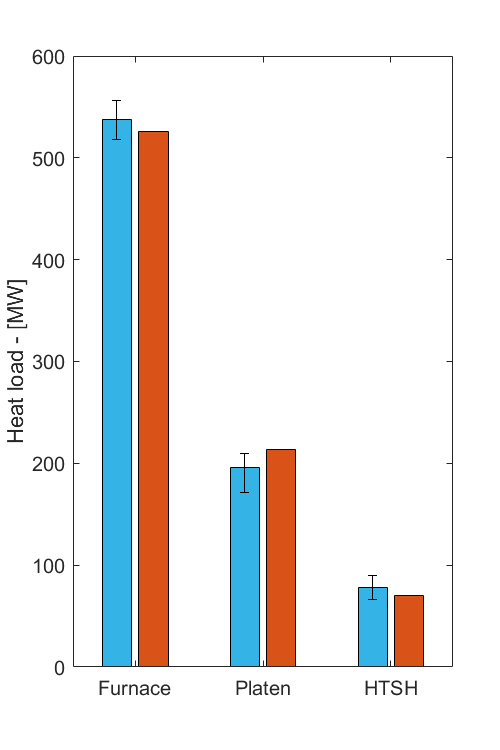
\includegraphics[width=0.32\textwidth]{100_VALID_BAR}}
	\subfigure[80 \% MCR]{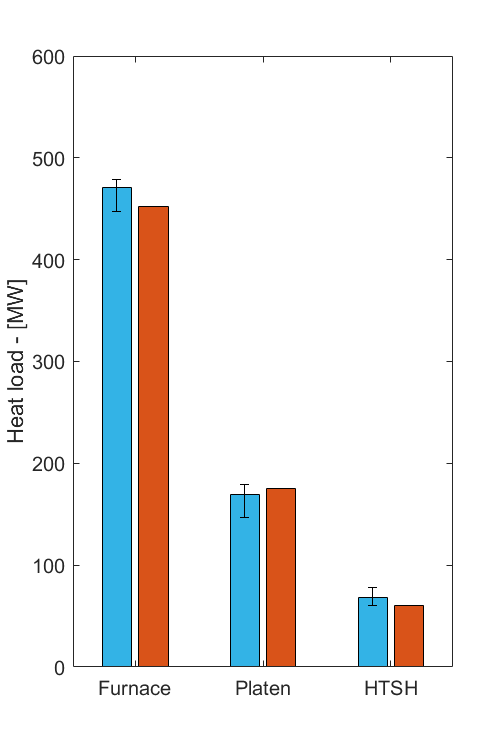
\includegraphics[width=0.32\textwidth]{80_VALID_BAR}}
	\subfigure[60 \% MCR]{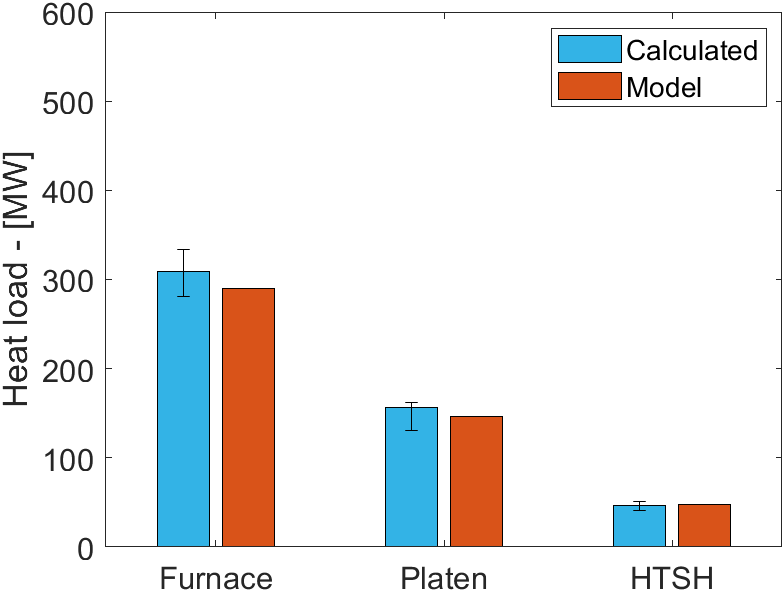
\includegraphics[width=0.32\textwidth]{60_VALID_BAR}}
\caption{Comparison of experimentally calculated and model heat loads for the furnace, platen SH and final SH}
\label{fig_heat_valid}
\end{figure}
\clearpage
In Figure \ref{fig_heat_valid} it is shown that the overall heat loads are in good agreement with the calculated results. For the simulated validation loads the proposed model results are within the associated error band, the general trend is an under prediction on the furnace heat loads, with a maximum percentage error of 2 \%, and an over prediction on the platen SH, with a maximum percentage error of 7 \% . The pendant SH illustrate the best comparable results for all load Cases.

The CFD model was further validated by comparing the $CO_{ppm}$ and $X_{O_{2}}$ measurements against the CFD results. The probe measurements were taken at a furnace height of 37.5 [$m$] near the center of the boiler during a full load (100\% MCR) operating conditions. The probe is inserted from the side walls to a depth of 4.5 [$m$], measurements were taken every 0.5 [$m$].\\
\begin{figure}[h!]
\centering
\subfigure[]{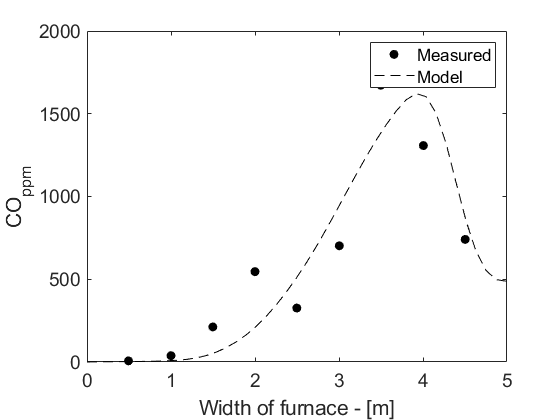
\includegraphics[width = 0.45\textwidth, height =4cm ]{COPPM_VALID}}
\hspace{5mm}
\subfigure[]{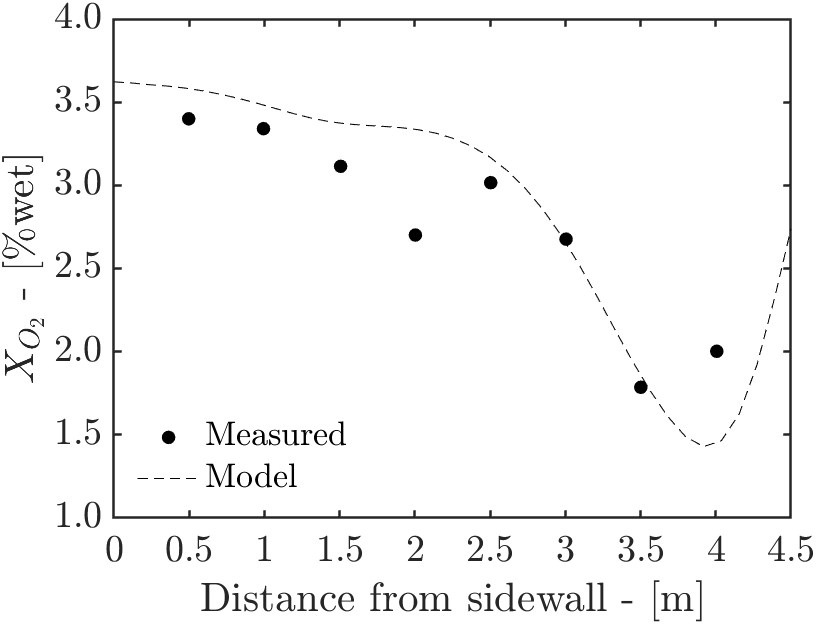
\includegraphics[width = 0.45\textwidth, height =4cm ]{XO2_VALID}}
\caption{Experimentally calculated $CO_{ppm}$ (a) and $X_{O_{2}}$ (b) concentration predictions}
\label{fig_probe_valid}
\end{figure}

Figure \ref{fig_probe_valid} shows the averaged measurement values compared to the CFD predictions. It can be seen that the CFD model can sufficiently resolve the $CO_{ppm}$ and $X_{O_{2}}$ concentrations at the given probe location.
\newpage
\subsection{Simulation results for various burner firing arrangements at 32\% MCR }
The temperature and velocity profiles for the various firing arrangements are shown in Figures \ref{fig_cfd_temp} and \ref{fig_cfd_velo} respectively. When the middle burner rows firing (Cases 2 and 5) a substantial cold region is formed in the lower half the furnace, resulting in the lowest heat uptake. This is further exacerbated when considering Table \ref{tbl_process_parameters} where it is illustrated that the mid-firing arrangements produce the lowest steam flow rates resulting in the lowest boiler efficiencies. The bottom firing arrangement (Cases 1 and 4) results in a high temperature zone located in the bottom half on the burner, while the mixed firing arrangement (Cases 3 and 6) results is an even distribution of high temperature gases across the furnace domain (Figure \ref{fig_cfd_temp}). This leads to the highest steam generation rate in the furnace and boiler efficiency as shown in Table \ref{tbl_process_parameters}.

\begin{figure}[h!]
\centering
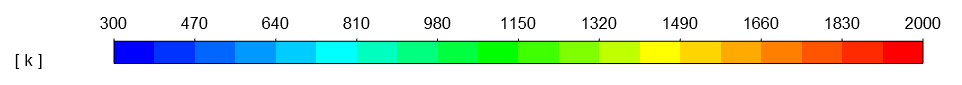
\includegraphics[scale = 0.45]{TEMP_KEY} [$K$]\\
\subfigure[Case 1]{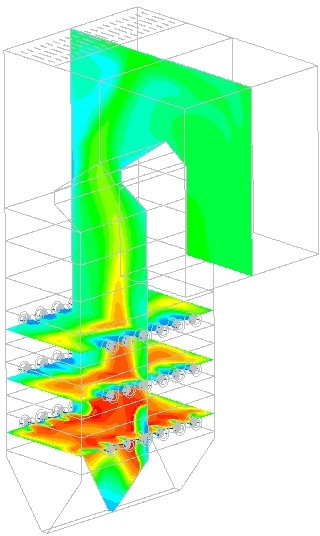
\includegraphics[width=0.32\textwidth]{BOT_TEMP}}
\subfigure[Case 2]{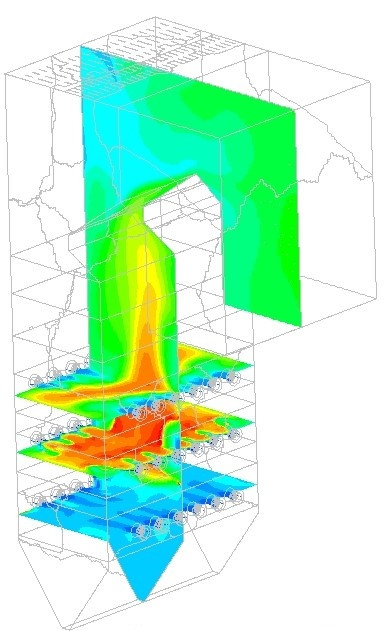
\includegraphics[width=0.32\textwidth]{MID_TEMP}}
\subfigure[Case 3]{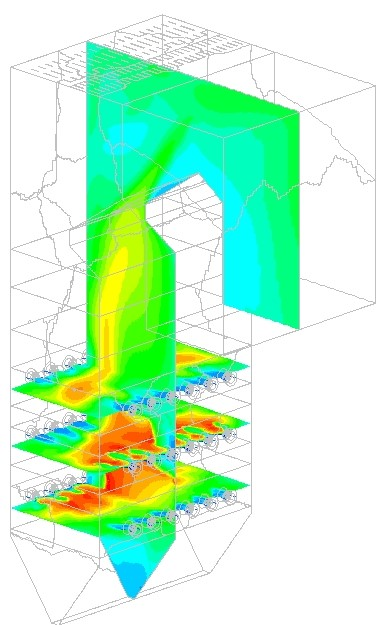
\includegraphics[width=0.32\textwidth]{FBRM_TEMP}}\\
\subfigure[Case 4]{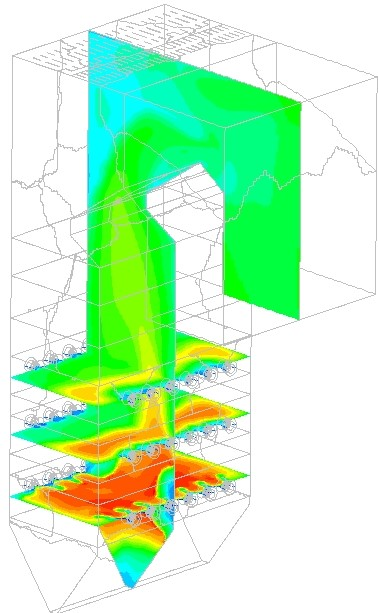
\includegraphics[width=0.32\textwidth]{BOT05_TEMP}}
\subfigure[Case 5]{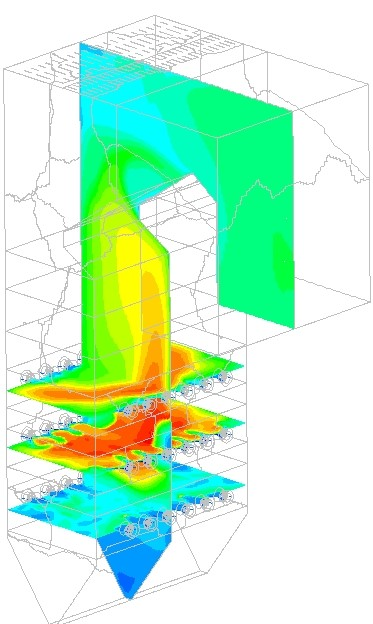
\includegraphics[width=0.32\textwidth]{MID05_TEMP}}
\subfigure[Case 6]{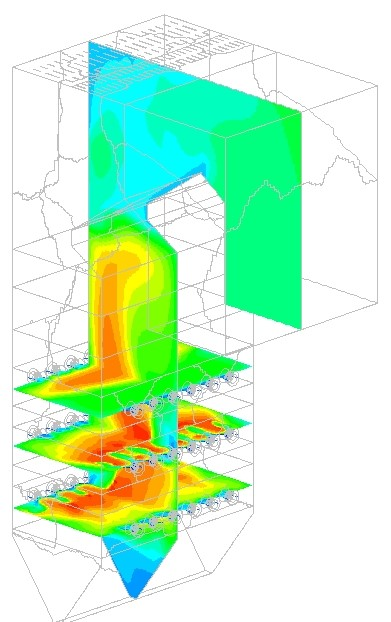
\includegraphics[width=0.32\textwidth]{FBRM05_TEMP}}
\caption{Temperature fields for Cases 1 through 6 [(a)-(f)]}
\label{fig_cfd_temp}
\end{figure}

\begin{figure}[h!]
\centering
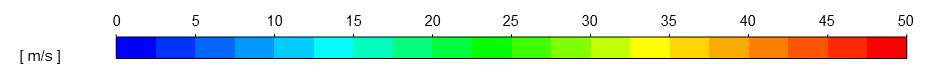
\includegraphics[scale = 0.45]{VEL_KEY} [$m/s$]\\
\subfigure[Case 1]{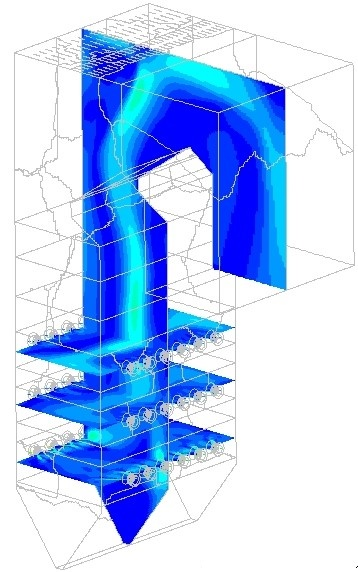
\includegraphics[width=0.32\textwidth]{BOT_VEL}}
\subfigure[Case 2]{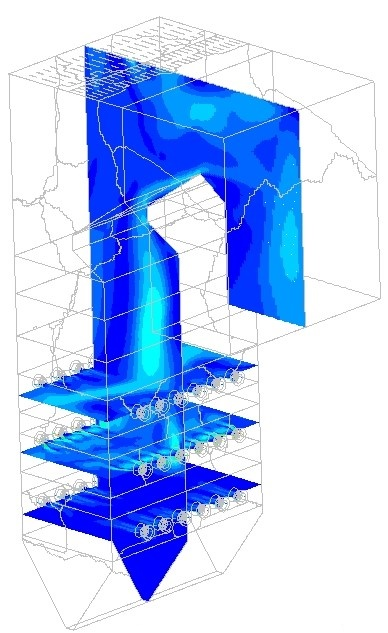
\includegraphics[width=0.32\textwidth]{MID_VEL}}
\subfigure[Case 3]{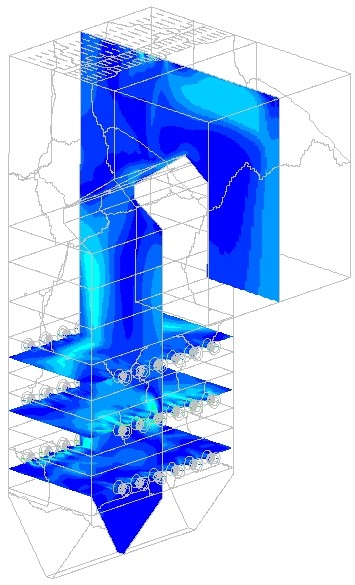
\includegraphics[width=0.32\textwidth]{FBRM_VEL}}\\
\subfigure[Case 4]{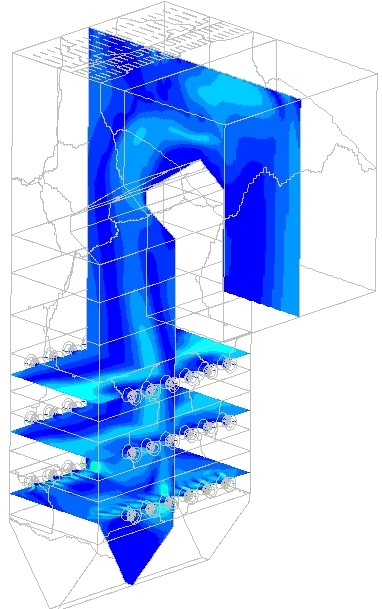
\includegraphics[width=0.32\textwidth]{BOT05_VEL}}
\subfigure[Case 5]{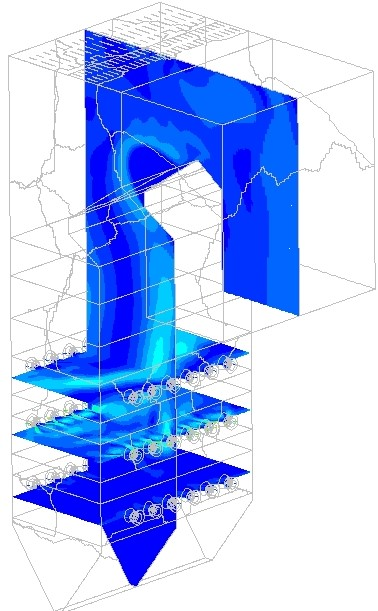
\includegraphics[width=0.32\textwidth]{MID05_VEL}}
\subfigure[Case 6]{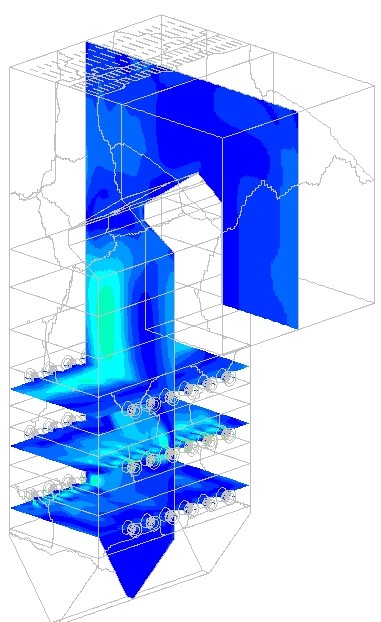
\includegraphics[width=0.32\textwidth]{FBRM05_VEL}}
\caption{Velocity fields for Cases 1 through 6 [(a)-(f)]}
\label{fig_cfd_velo}
\end{figure}

\begin{table}[h!]
\centering
\caption{Process model control parameters}
\vspace{2mm}
{\tabulinesep=1.2mm
\begin{tabularx}{\linewidth}{p{0.45\linewidth} XXXXXX}
\hline
&\multicolumn{6}{c}{Cases}\\
 & \textbf{1} & \textbf{2} & \textbf{3}& \textbf{4}&\textbf{5}&\textbf{6}\\
\hline
\textbf{Main steam flow-rate} 	[$kg/s$]		&175.8&172.9&180.5&180.2&179.1&184.1 \\
\textbf{Main steam exit temp} 	[$^{\circ}C$]	&535& 535 &535&535 &535& 535\\
\textbf{RH steam flow rate} 	[$kg/s$]		&158.2&155.6&162.5&162.2&161.2&165.6\\
\textbf{RH steam exit temp} 	[$^{\circ}C$]	&524&527&531&512&510&520\\
\textbf{Boiler efficiency} 		[$\%$]			&85.3&84.1&87.9	&87.2&85.9&89.1\\
\textbf{ATT1} 		[$kg/s$]					&10.4&16.9&13.9&7.9&5.5&10.9\\
\textbf{ATT2} 		[$kg/s$]					&1.7&3.8&4.2&3.8&3.6&4.2\\
\textbf{ATT-RH} 		[$kg/s$]				&0.0&0.0&0.0&0.0&0.0&0.0\\
\hline
\label{tbl_process_parameters}
\end{tabularx}}
\end{table}

Figure \ref{fig_cfd_heat_flux} illustrates the heat flux profiles for the simulated cases. Both cases 1 and 4 highlight high heat flux zones near the burner inlets which, in the presence of high temperatures and incomplete combustion near these regions, can lead to high-temperature corrosion \cite{Du2017}. An even distribution of unit heat fluxes is seen in Cases 3 and 6 with minimal localised heat flux concentrations being observed. Cases 2 and 5 show that most of the unit heat fluxes are absorbed in the upper half of the boiler with case 5 showing a higher heat flux on the rear wall. This could be due the use of a lower SA flow-rate leading to higher velocity profiles developing closer to the rear wall, as seen in Figure \ref{fig_cfd_velo}. With this is mind a lower SA flow-rate, in general leads to hot gases and velocity profiles impinging closer to the furnace walls, which can be seen in Cases 4, 5 and 6 of Figures \ref{fig_cfd_temp} and \ref{fig_cfd_velo} respectively. With high gas temperatures and high velocity impingement, Cases 4, 5 and 6 (of Figure \ref{fig_cfd_heat_flux}) experience concentrated heat fluxes around the burner inlets in comparison to corresponding Cases 1, 2 and 3.

\begin{figure}[h!]
\centering
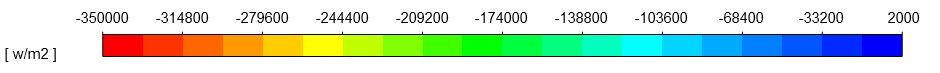
\includegraphics[scale = 0.45]{HEATFLUX_KEY} [$W/m^2$]\\
\subfigure[Case 1]{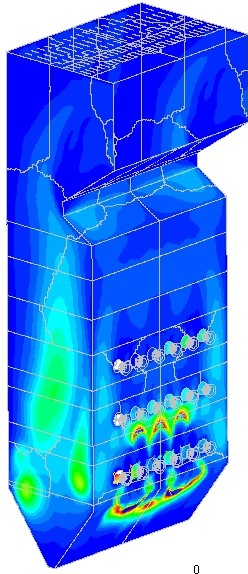
\includegraphics[scale = 0.35]{BOT_HEATFLUX}}
\hspace{5mm}
\subfigure[Case 2]{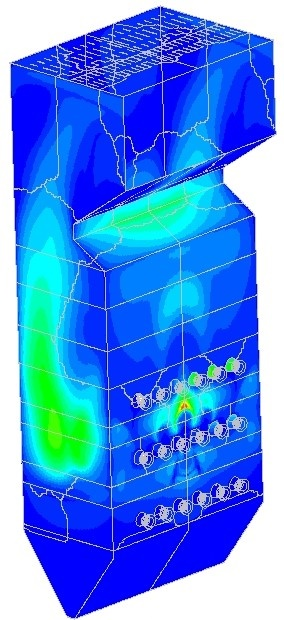
\includegraphics[scale = 0.35]{MID_HEATFLUX}}
\hspace{5mm}
\subfigure[Case 3]{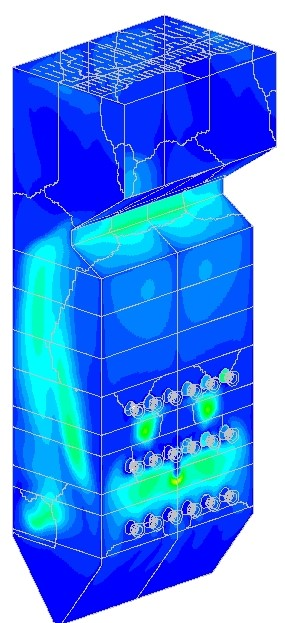
\includegraphics[scale = 0.35]{FBRM_HEATFLUX}}\\
\subfigure[Case 4]{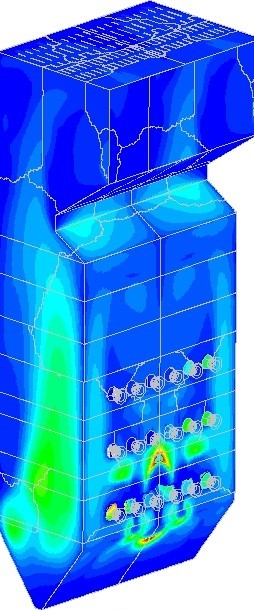
\includegraphics[scale = 0.29]{BOT05_HEATFLUX}}
\hspace{5mm}
\subfigure[Case 5]{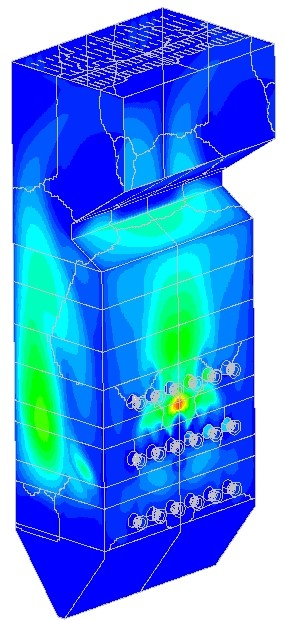
\includegraphics[scale = 0.35]{MID05_HEATFLUX}}
\hspace{5mm}
\subfigure[Case 6]{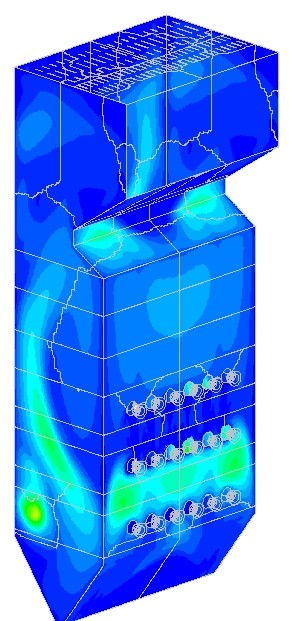
\includegraphics[scale = 0.35]{FBRM05_HEATFLUX}}
\caption{Heat fluxes profiles for Cases 1 through 6 [(a)-(f)]}
\label{fig_cfd_heat_flux}
\end{figure}

The works of Dugum et al \citep{Du2017}, highlights the issue of high-temperature corrosion caused by significant levels of $CO$ ($X_{CO}$ 0.01 - 0.1) and no-free $O_2$ near regions of high wall temperatures. For low-load operation this phenomena becomes important to avoid since combustion instability can lead to these non-ideal circumstances. Figure \ref{fig_cfd_coppm} shows the $CO$ molar concentration in the domain located on an iso-surface set 1600 $[K]$. The figures generally highlight the location and distribution of the flame core for each case. Cases 1 and 4 illustrate the highest likelihood of high-temperature corrosion occurring near the furnace hopper, due to the high concentration and temperatures in that region.

\begin{figure}[h!]
\centering
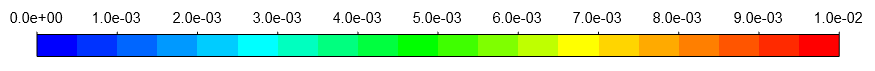
\includegraphics[scale=0.45]{CO_MF_KEY} [$X_{CO}$] \\
\subfigure[Case 1]{	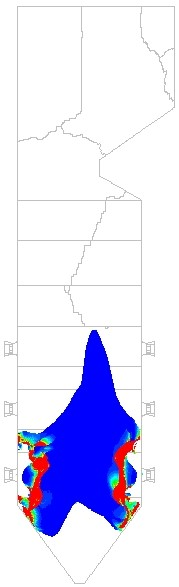
\includegraphics[width=0.18\textwidth, height = 7cm]{BOT_ISO_COPPM_F}
				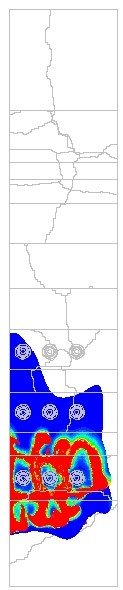
\includegraphics[height = 7cm]{BOT_ISO_COPPM_S}}
\subfigure[Case 2]{	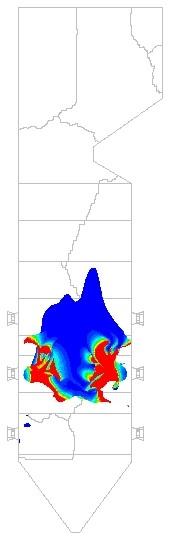
\includegraphics[width=0.18\textwidth, height = 7cm]{MID_ISO_COPPM_F}
				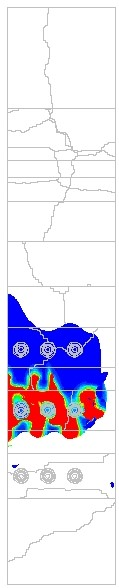
\includegraphics[height = 7cm]{MID_ISO_COPPM_S}}
\subfigure[Case 3]{	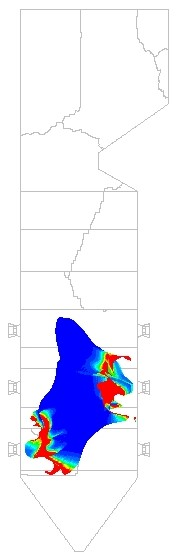
\includegraphics[width=0.18\textwidth, height = 7cm]{FBRM_ISO_COPPM_F}
				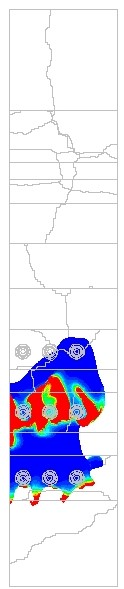
\includegraphics[height = 7cm]{FBRM_ISO_COPPM_S}}\\
\subfigure[Case 4]{	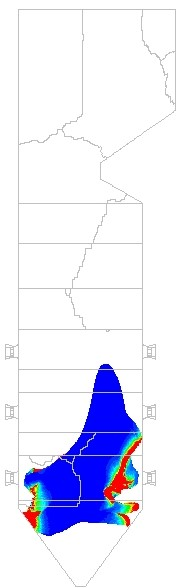
\includegraphics[width=0.18\textwidth, height = 7cm]{BOT05_ISO_COPPM_F}
				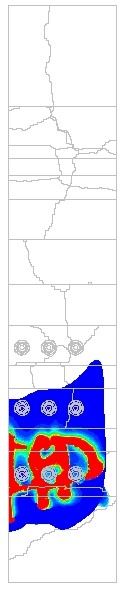
\includegraphics[height = 7cm]{BOT05_ISO_COPPM_S}}
\subfigure[Case 5]{	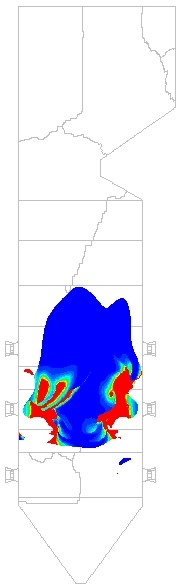
\includegraphics[width=0.18\textwidth, height = 7cm]{MID05_ISO_COPPM_F}
				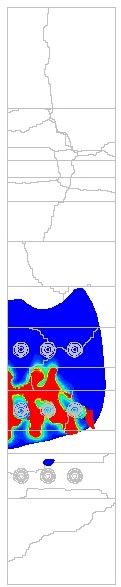
\includegraphics[height = 7cm]{MID05_ISO_COPPM_S}}
\subfigure[Case 6]{	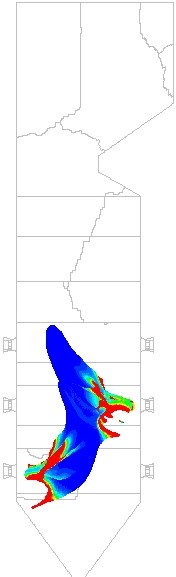
\includegraphics[width=0.18\textwidth, height = 7cm]{FBRM05_ISO_COPPM_F}
				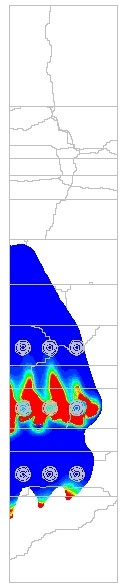
\includegraphics[height = 7cm]{FBRM05_ISO_COPPM_S}}\\
\caption{CO molar fraction ($X_{CO}$) concentrations for 
Cases 1 through 6 [(a)-(f)] on a temperature iso-surface of 1600 [K]}
\label{fig_cfd_coppm}
\end{figure}

Investigating the combustion stability for all the Cases, the symmetry and offset vertical probe plots (as highlighted in Figure \ref{fig_geometry}) are given in Figure \ref{fig_cfd_probe}. Cases 2 and 5 illustrates the highest $X_{O_{2}}$ concentration in the lower half of the burner since there is minimal combustion occurring. The unburnt carbon content and exit flue-gas temperatures for each case are reported in Table \ref{tbl_cfd_results}. With the use of the middle burners (Cases 2 and 5) the highest exit temperature and unburnt carbon content is observed, since the flame core is located in the upper half of the furnace leading to the least possibility of complete combustion due to the shorter residence time. Cases 3 and 6 exhibit the best characteristics with the least amount of unburnt carbon content being observed. It is important to note the effects of a lower SA mass flow rate has on the furnace exit conditions for non-firing burners which generally leads to a hotter exit gas temperature as seen with Cases 4 to 6. 

\begin{figure}[h!]
\centering
\subfigure[Symmetry vertical plot]{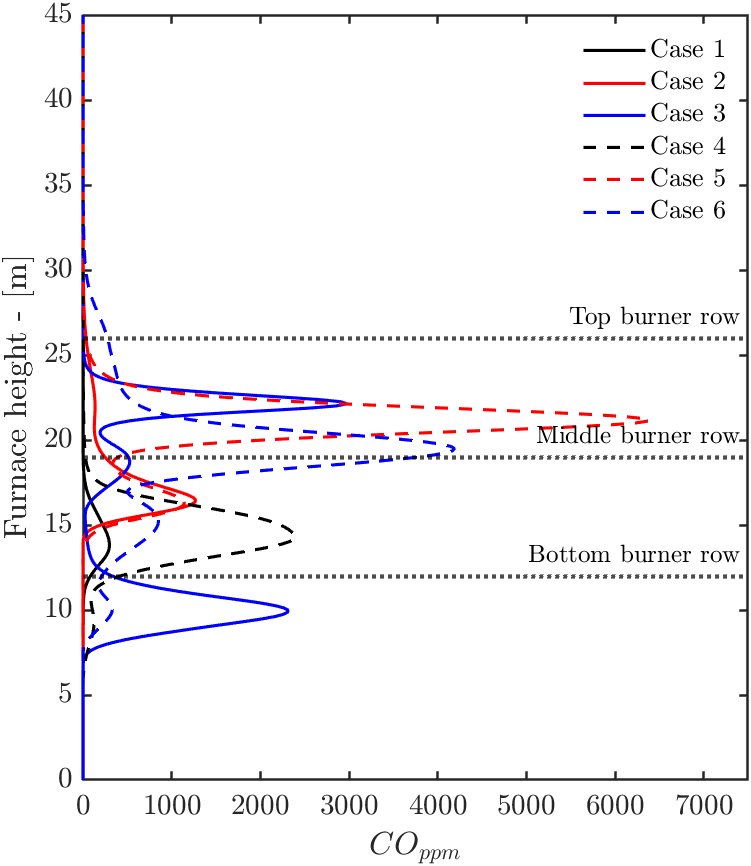
\includegraphics[scale = 0.36]{SYMMETRY_PROBE_COPPM}}
\hspace{5mm}
\subfigure[Offset vertical plot]{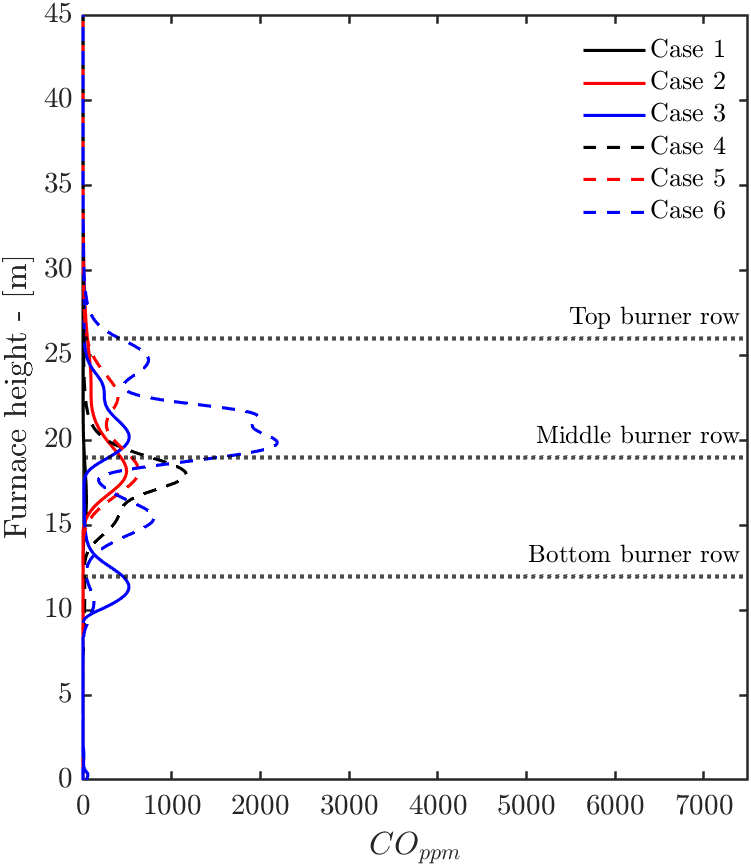
\includegraphics[scale = 0.36]{OFFSET_PROBE_COPPM}}\\
\subfigure[Symmetry vertical plot]{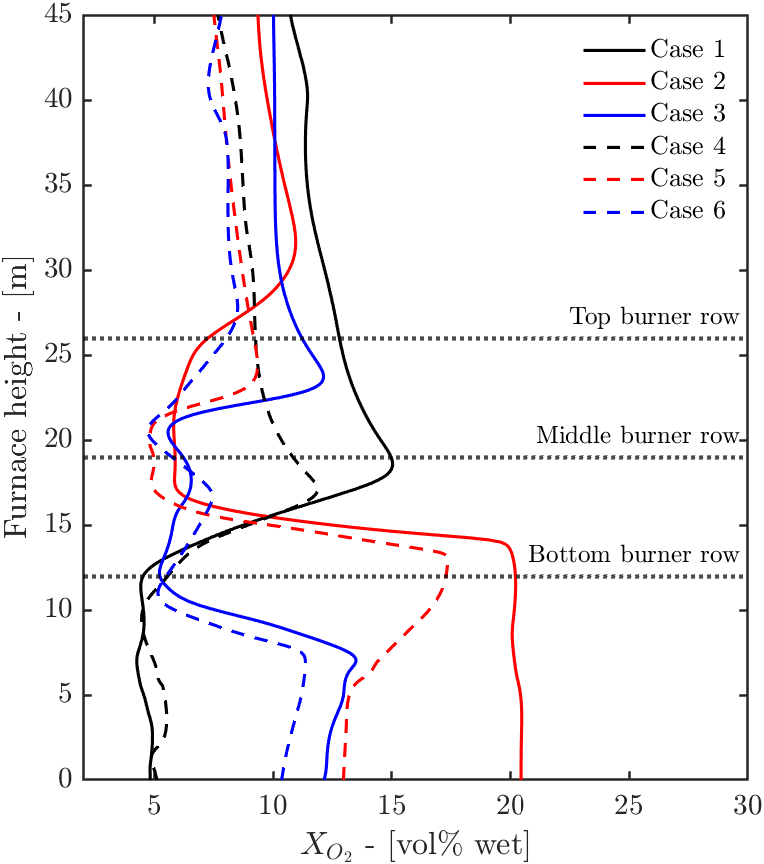
\includegraphics[scale = 0.35]{SYMMETRY_PROBE_XO2}}
\hspace{5mm}
\subfigure[Offset vertical plot]{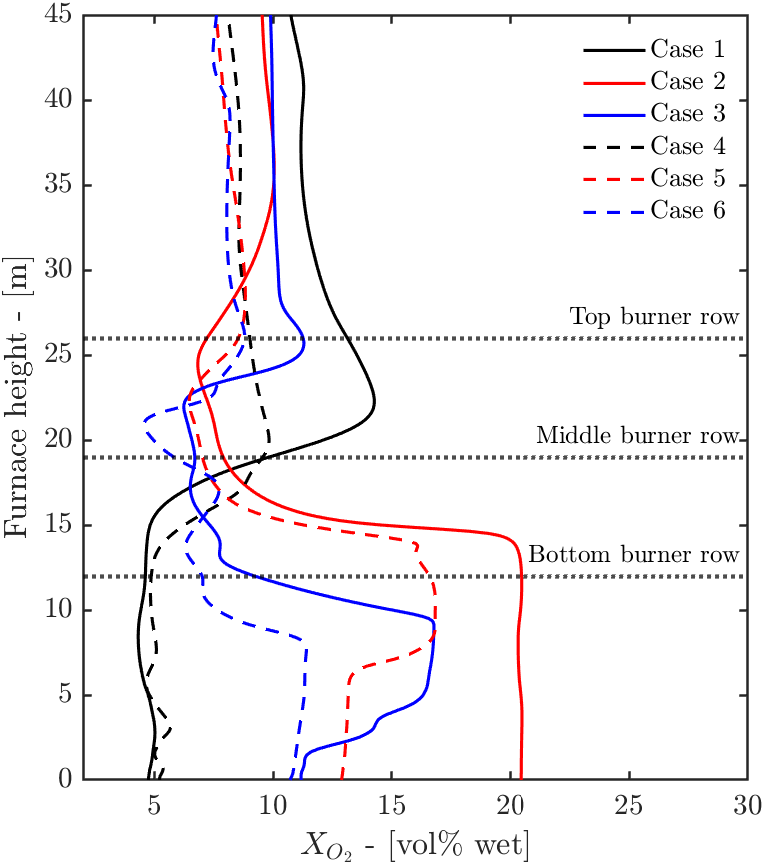
\includegraphics[scale = 0.35]{OFFSET_PROBE_XO2}}
\caption{$CO_{PPM}$ [(a) and (b)] and $X_{O_{2}}$ [(c) and (d)] line plots on symmetry and offset vertical probe lines}
\label{fig_cfd_probe}
\end{figure}
\clearpage

\begin{table}[h!]
\centering
\caption{Furnace exit conditions and SH wall temperatures}
\vspace{2mm}
{\tabulinesep=1.2mm
\begin{tabularx}{\linewidth}{p{0.4\linewidth} XXXXXX}
\hline
&\multicolumn{6}{c}{Cases}\\
 & \textbf{1} & \textbf{2} & \textbf{3}& \textbf{4}&\textbf{5}&\textbf{6}\\
\hline
\multicolumn{7}{l}{\textit{Furnace exit}}\\
\textbf{Exit temperature} [$K$] & 1168 & 1230 & 1215 & 1208 & 1306 & 1298\\
\textbf{Unburnt carbon} [$(\times 10^{-3})\,\%$] & 1.83 & 1.94 & 1.54 & 1.81 & 1.89 & 1.62\\
\multicolumn{7}{l}{\textit{Platen SH}}\\
\textbf{Max wall temperature} [$^{\circ}C$]  &477 & 492 & 481  & 480 & 493 & 490\\
\textbf{Mean wall temperature} [$^{\circ}C$] &439 & 453 & 446 & 454 & 442 & 451\\
\multicolumn{7}{l}{\textit{Final SH}}\\
\textbf{Max wall temperature} [$^{\circ}C$]  & 602 & 624 & 608 & 595 & 626 & 612\\
\textbf{Mean wall temperature} [$^{\circ}C$] & 520 & 523 & 517 & 512 & 520 & 511\\
\hline
\label{tbl_cfd_results}
\end{tabularx}}
\end{table}
The external tube metal temperatures, of Table \ref{tbl_cfd_results}, were calculated using equation \ref{eqn_t_wall}, which takes into account the temperature drop due to the ash deposit present on platen and final SH. Fouling thermal resistances of 0.0067 and 0.015 [$m^2K/W$] were used for the platen and final SH respectively.  
\begin{equation}\label{eqn_t_wall}
T_{metal} = T_{wall} - \left(\frac{\dot{q}_{SH}t_{ASH}}{\lambda_{ASH}}\right)
\end{equation}
For the platen and final SH the maximum surface temperature are observed for Cases 2 and 5. For comparison at 100 \% MCR load the maximum and mean temperatures reported for the platen and final SH are 500 \& 446 $[^\circ C]$ and 623 \& 531 $[^\circ C]$ respectively, with the final SH operating in the materials creep range \cite{Laubscher2019b}. Thus, continued operation using the firing arrangement of Cases 2 and 5, could lead to SH failure.

Using the process model of Figure \ref{fig_flownex} and the results of the CFD simulations the important process control parameters were determined. Table \ref{tbl_process_parameters} summarizes the results with the highest boiler efficiencies observed for Cases 3 and 6. With a lower SA flow-rate Cases 4 to 6 exhibit a higher boiler efficiency due to the decrease in dry gas losses, when compared to Cases 1 to 3. All Cases exhibit adequate control of the main steam exit temperature by use of ATT1 and ATT2. The exit temperature of the reheaters, for all Cases, are determined to within the 20 [$^\circ C$] tolerance for the intermediate turbine inlet conditions, as stipulated in the design C-schedules for the plant. However, with the lack of ATT-RH control, a sudden decreases in steam generation can lead to RH overheating and possible RH failure. Considering all of the above, Cases 3 and 6 are seen as the best firing arrangements for continuous low-load operation at a load 32 \% MCR.

Table \ref{tbl_rad_conv} shows the radiative heat percentage of the total heat input into each heat exchanger for Cases 3 and 6. It can be seen that heat transfer to the furnace and radiant SHs are dominated by radiation, with approximately $\pm$ 10 \% being transferred to convection at low-load. Considering the convective pass heat exchangers (RH2 through to the EC, refer to Figure \ref{fig_flownex}) the convective heat transfer becomes more apparent as seen with the reduction in radiative heat transfer percentage. Case 6 tends to exhibit less convective heat transfer for the said  heat exchangers, due to the fact of a lower SA flow-rate for non-firing burners. This will reduce the total amount of flue-gas flowing through the boiler, for the same cross flow-area and similar density the velocity would be expected to drop, reducing the convective heat transfer.

\begin{table}[h!]
\centering
\caption{Radiative heat transfer percentage for Cases 3 and 6}
\vspace{2mm}
{\tabulinesep=1.2mm
\begin{tabularx}{\linewidth}{p{0.4\linewidth} XX}
\hline
 &\textbf{Case 3}&\textbf{Case 6}\\
\hline
Furnace [\%] & 89.2 & 88.9\\
Platen SH (SH2) [\%] & 92.5& 93.4\\
Final SH (SH3) [\%] & 93.5& 94.0\\
RH2 [\%] & 47.6& 52.2\\
SH1 [\%] & 37.2& 40.7\\
RH1 [\%] & 18.7& 21.5\\
EC [\%] & 5.4& 6.5\\
\hline
\label{tbl_rad_conv}
\end{tabularx}}
\end{table}

\clearpage
\section{Conclusions}
The present study demonstrates the use of a coupled simulation used to study the effects of burner configuration at a boiler load of 32 \% MCR. A validation case was performed for the developed CFD model which showed adequate results for heat fluxes to the walls, with a general tendency of the model to under-predict the heat fluxes to the furnace. The model also showed sufficient accuracy in determining the combustion characteristics at the 100 \% MCR load. 

The results show that using a burner arrangement that raises the position of the flame core (Cases 2 and 5) increases the exit flue-gas temperature and runs the risk of final SH failure due to overheating. Subsequently, this firing arrangement also results in a higher unburnt carbon percentage at the exit flue-gas stream potentially leading to economic losses, regarding the efficient combustion of the fuel and the lowest boiler utilization efficiency.

Operation of the boiler using firing arrangements of Cases 1 and 4, in relation to Cases 3 and 6 results in lower boiler utilization efficiency and exit flue-gas temperature. Higher $X_{CO}$ concentrations are observed near the bottom half of the furnace, along with high temperatures, which can lead to a high possibility of fire side corrosion occurring at continuous low-load operation using Cases 1 and 4.

The mixed firing arrangement, of case 3 and 6, exhibits the best boiler utilization efficiency overall. A 4.8 \% decrease in unburnt carbon percentage is observed when operating using case 3 in relation to case 6. The predicted re-heater exit steam temperature of case 3 is substantially closer to the desired the temperature of 535 $[^\circ C]$, allowing for better control. 

Based on the current numerical study, carried out to determine the most favourable operating parameters and combustion stability, case 3 is seen as the optimal firing arrangement for the boiler under consideration.

\section*{Acknowledgements}
The authors would like to thank the Eskom EPPEI program for financially supporting the present study and acknowledge the computational resources provided by the Centre for High Performance Computing (CHPC), South Africa.

\bibliography{PAPER1_LOW_LOAD}

\end{document}
